\section{Basics}

\begin{frame}{Experimental Setup}
  \begin{bigidea}{Methode}
      Spinning molecules in superfluid helium nanodroplets with an optical centrifuge.
    \end{bigidea}
    \twocol{
      \begin{block}{Centrifuge}
        \begin{itemize}
          \item two circular polarized chirped pulses
          \item interference gives rotating linear polarization
          \item adaptable acceleration possible
        \end{itemize}
      \end{block}
    }{\begin{block}{Droplets}
        \begin{itemize}
          \item expansion through cooled nozzle
          \item temperature around $0.4\, \mathrm{K}$
          \item radius $10-100\, \mathrm{nm}$
          \item doped with single molecules
        \end{itemize}
      \end{block}}
\end{frame}

\begin{frame}{What do we measure?}
  \begin{block}{$\langle cos^2(\Theta_{\mathrm{2D}})\rangle$ against $\mathrm{probe\, delay}$}
    \begin{figure}
    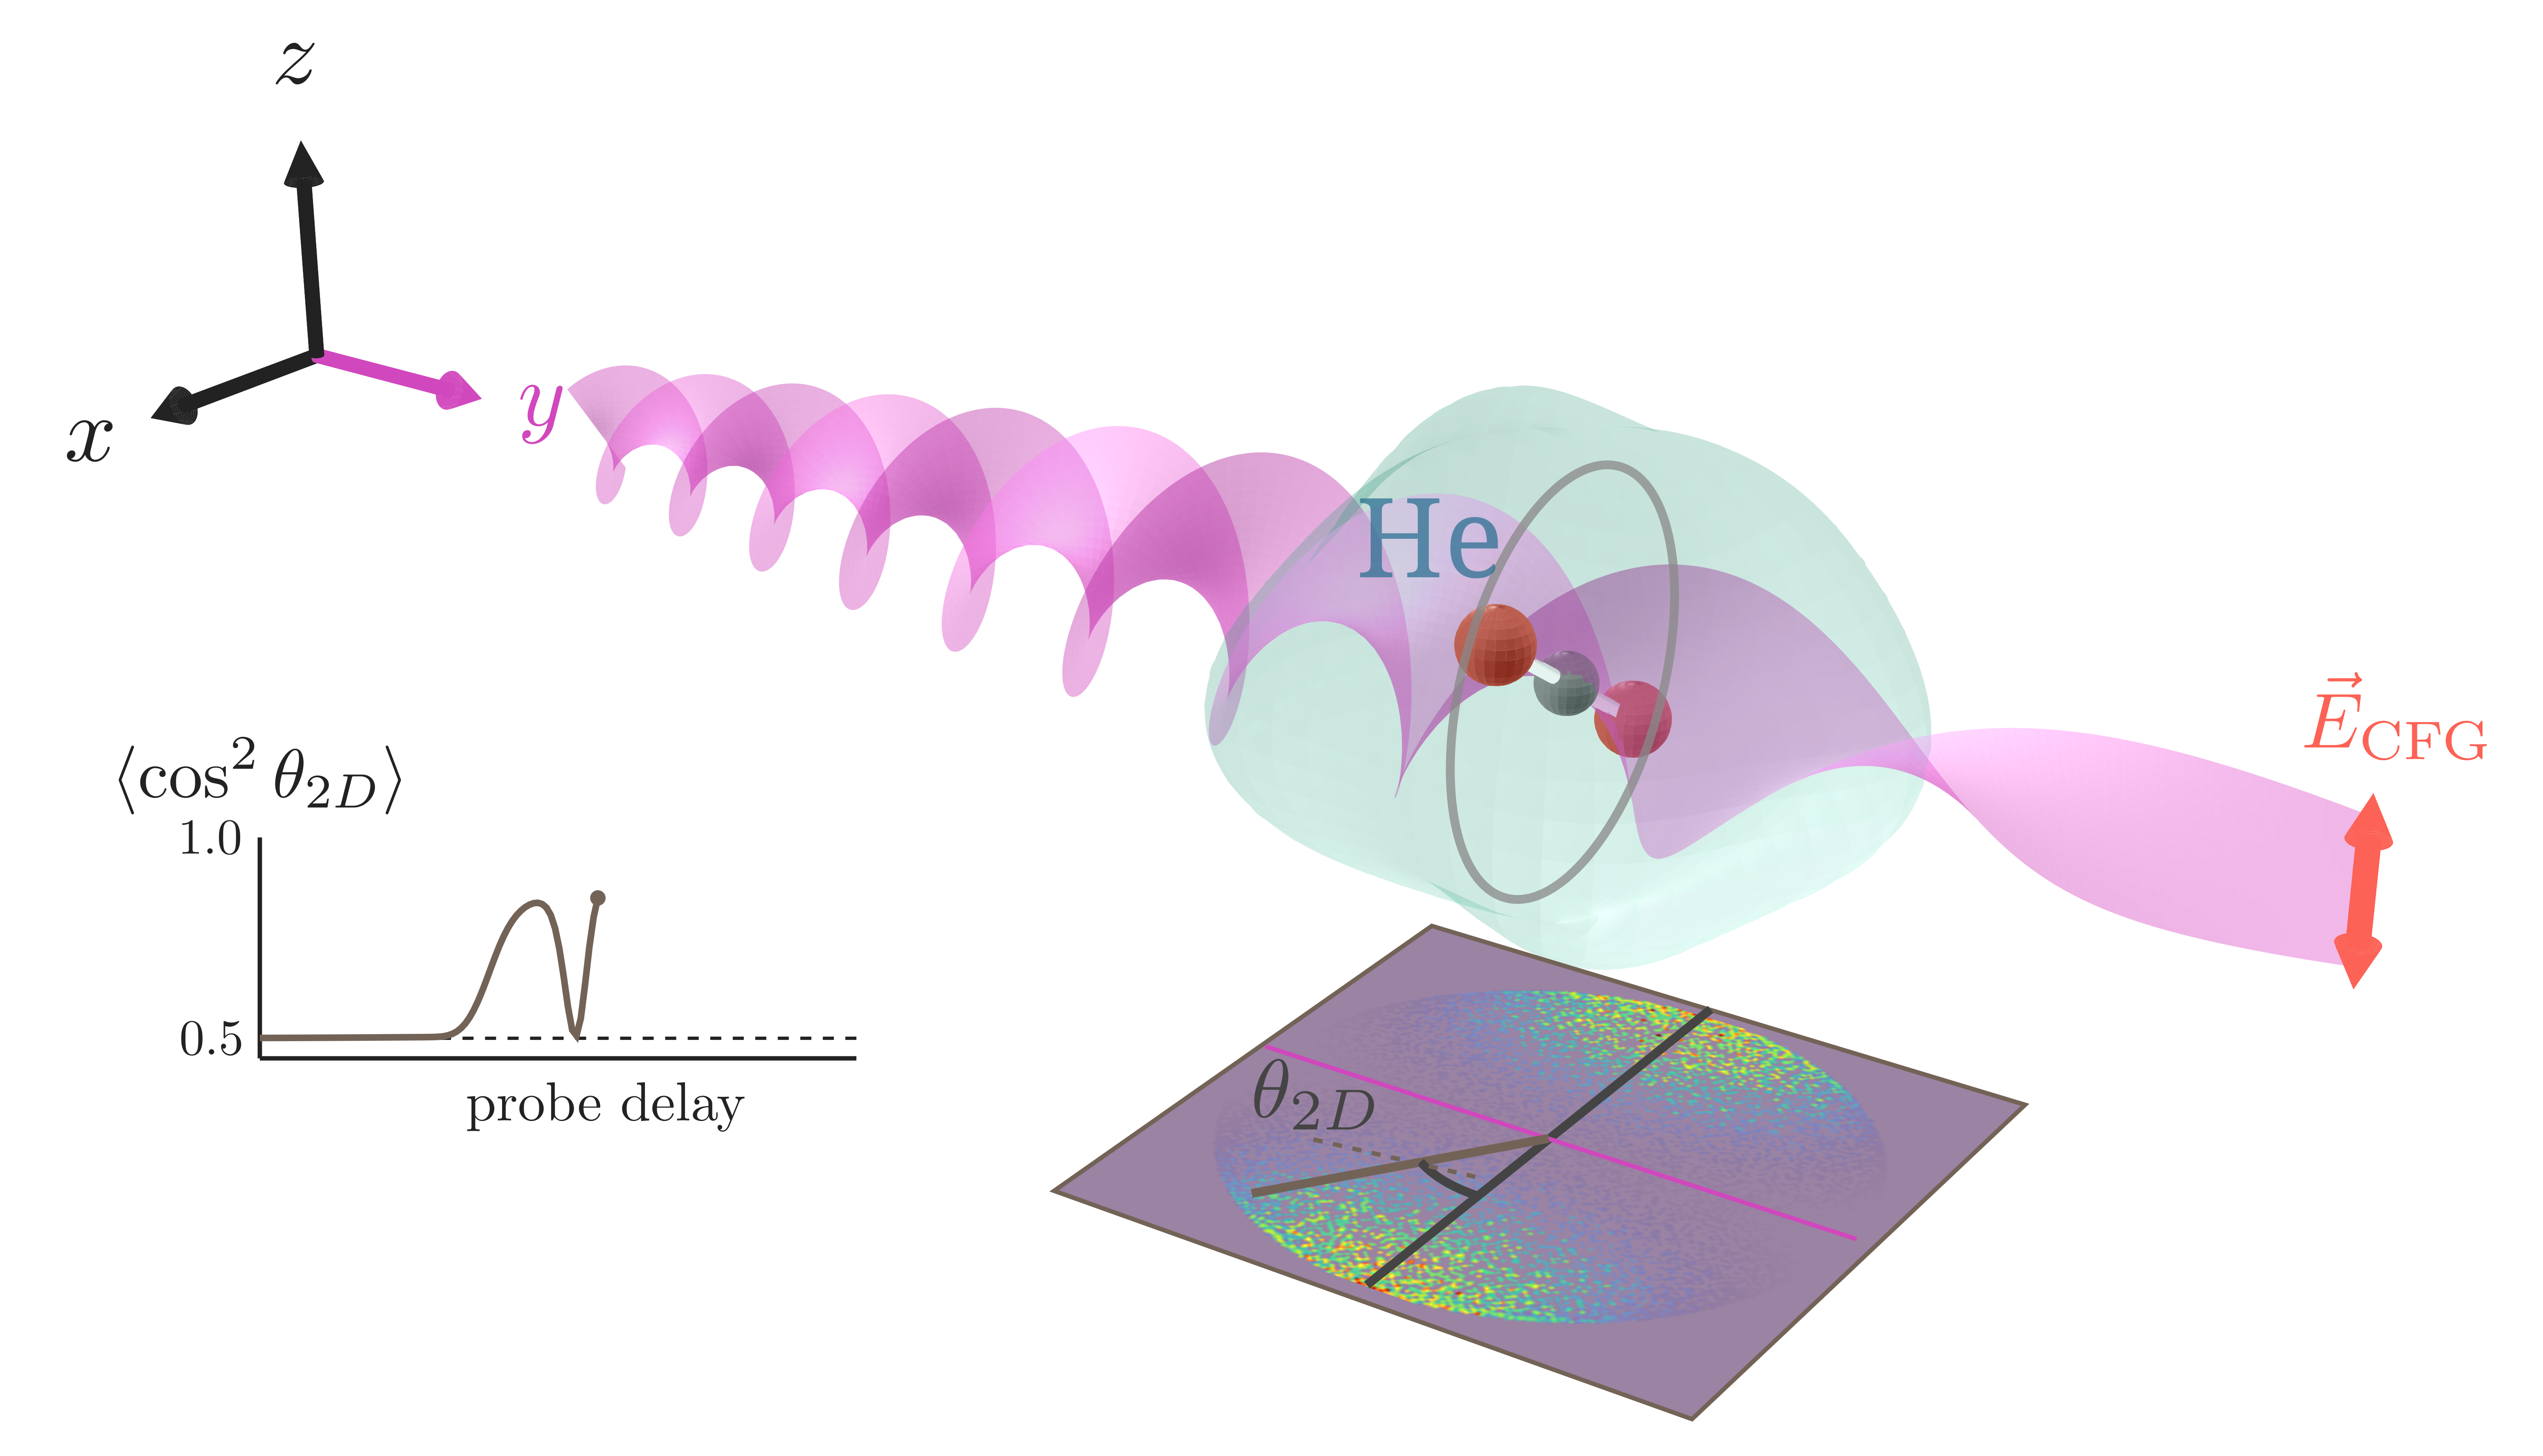
\includegraphics[width=0.7\linewidth]{figures/cfg_setup.png}
  \end{figure}
  \end{block}
\end{frame}

\begin{frame}{Centrifuge-Molecule interaction}
  \textbf{Centrifuge-Molecule potential}:
  \[
  \boxed{
    V_{\mathrm{drive}} \propto
    -\Delta\alpha E^2(t)\cos^2(\theta)
  }
\]
  where
\[
\begin{array}{@{}ll@{}}
  \Delta \alpha = \alpha_{\parallel}-\alpha_{\perp}
    & \text{anisotropic polarizability} \\
  E(t)
    & \text{Gaussian pulse envelope} \\
  \theta
    & \text{angle between the polarization axis and the E-field}
\end{array}
\]
\vspace{0.05cm}
\noindent\rule{\linewidth}{0.5pt}
\vspace{0.05cm}
\textbf{Spinnability}:
\[
  \boxed{
    \sigma_0 := \frac{V_0}{\pi I \beta}
  }
\]
where
\[
\begin{array}{@{}ll@{}}
  I
    & \text{moment of inertia} \\
  \beta
    & \text{acceleration of the centrifuge}
\end{array}
\]
\end{frame}